\chapter{Introduction --- orthography}
\label{cha:intr-orth}

In Part~\ref{part:phonology-phonetics}, I argue that \lT\ and \xD\ were phonologically distinct at least until and including the period up until the thirteenth century when the Poets of the Princes were active. In this Part, I argue that this phonological distinction affected the orthography of lenition well into the \gls{mw} period, which lasted until the fifteenth century. More specifically, I will demonstrate that word-initial lenition of \mw[]{p, t, c} was not written until about 1300%
\footnote{I consider \mw[]{k} an allograph of \mw[]{c} for the purpose of lenition; therefore it i obvious that lenition of \mw[]{k} was not written either.}.
Thus, there existed a time from the \gls{ow} period up until this point when lenition of  voiceless stops was not written word-initially, even though lenition of most other consonants was.

Orthographical representation of lenition of most consonats arose at the end of the \gls{ow} period. At this time, the distinction between \lT\ and \xD\ was still maintained; and as a result, scribes struggled to represent the existence of three different stop series \xT, \lT, and \xD, because the Latin alphabet  provides not three but two sets of stop consonants. This made it impossible to keep apart in writing all three stop series that Welsh had at the time%
\footnote{Similar trouble existed for fricatives. For instance, \textcite[28]{russell_rowynniauc_2003} notes that `[i]t has long been observed that, because of the rise of fricatives and spirants within the history of British, early Welsh was seriously understocked in signs to represent the full consonantal inventory.'}.

Word-initially, no natural association existed between \lT\ and \xD\ until the point when they merged phonologically, so the natural result of this phonology and the limitations of the Latin alphabet was for lenited voiceless stops to be written with \mw[]{p, t, c}; thus, early \gls{mw} orthography represented lenition only for consonants other than voiceless stops\footnote{Of course, lenition was not written for \mw{d} and \mw{rh} either, but orthographical representation for those consonants only became standard by the end of the \gls{mw} period.}.

\section{Textual evidence}
\label{sec:two-exampl-mowm}
MS \gls{sA}, the Black Book of Chirk,  is an example of a manuscript employing this limited orthographical system of lenition, as is illustrated in Example~\ref{ex:aylodeubrenyna}: 
\mwcc[ex:aylodeubrenyna]{\gls{sA}~4.9--10}{sef eu aylodeu e brenyn. \al{y u}eybyon ay neyeynt a\al{y k}euenderu.}{These are the members of the king: his sons and his nephews and his cousin.}
Here, lenition is represented following  \mw[his]{y} in \mw[sons]{ueybyon}, from unlenited \mw[]{meybyon}, but not in \mw[cousin]{keuenderu}, even though \mw{y} must obviously be translated as `his' before both words. In this example, the parallel construction makes it obvious that \mw[]{keuenderu} should be lenited, even though  no orthographical lenition backs this up.

The fact that lenited \mw[]{p, t, c} are written exactly the same as their radical counterparts makes it difficult to identify the exact geographical and chronological extent to which the non-merger of \xD\ and \lT\ existed. The only way to identify this non-merger is usually by observing the places in a \gls{mw} text where we would expect lenition, but where it is not written. Naturally, these identifications require thorough knowledge of lenition in  the grammar of early \gls{mw}\footnote{In Chapter~\ref{cha:some-phon-issu} I discuss my policy on where lenition can consistently be expected, and in Appendix~\ref{cha:database-lenition} I give a concrete list of leniting environments.}. Fortunately, the early convention where lenition of voiceless stops is not written can be discerned in a few cases, even in the absence of such thorough knowledge. The existence of an early \gls{mw} period with orthographic lenition, but  not of \lT, may be established even without knowledge of when exactly to expect lenition, based on two manuscript copies of the elegy of Madog ap Maredudd  by Cynddelw Brydydd Mawr. Example~\ref{ex:marwnadcomparison} shows the opening lines of this poem as they are found in \gls{bbc}  and \gls{h}, respectively.
\begin{mwl}
\item%
  \begin{minipage}[t]{0.45\textwidth}
    \mw{%
      Kẏwarchaw im ri.\ rad wobeith.\\
      Kẏwarchaw kẏwercheiſ e \al{c}anweith.\\
      Ẏ \al{p}rowi prẏdv.\ o\abbr{m} priwieth eurgert.\\
      ẏm argluit \al{k}edẏmteith.\\
      Ẏ \al{c}vinav madauc.\ metweith ẏ alar\\
      ae alon ẏm pop ieith.\\
      Doꝛ yſgoꝛ ẏſcvid \al{c}anhimteith.}\\
    (\acrshort{bbc}~52v.3--7)
  \end{minipage}~
  \begin{minipage}[t]{0.45\textwidth}
    \mw{%
      Kẏuarchaf ẏm ri rad o obeith.\\
      kẏuarchaf, kẏuercheis \al{g}anweith.\\
      ẏ \al{b}ꝛoui pꝛẏdu om pꝛifẏeith eurgert.\\
      ẏm arglwẏt \al{g}edymdeith.\\
      ẏ \al{G}wẏnaỽ madaỽc metueith.\ ẏ alar\\
      ae alon ẏm pob ẏeith\\
      Doꝛ ẏſgoꝛ ẏſgwẏd \al{g}anhẏmdeith.}\\
    (\acrshort{h}~47v.8--13)
  \end{minipage}
  \label{ex:marwnadcomparison}
\end{mwl}
Here,  lenition is written in \gls{bbc} to some extent, \eg in \mw[mourning him]{ẏ alar}, but wherever lenition  of \mw[]{p, t, c} is written in \gls{h}, the radical consonant is found in \gls{bbc}. These instances are marked in Example~\ref{ex:marwnadcomparison}. Note that word-medial lenition of voiceless stops does not necessarily differ between \gls{bbc} and \gls{h}, \cf \mw[golden song]{eur\al{g}ert} in both manuscripts, but \mw[companion]{kedẏm\al{t}eith/gedym\al{d}eith} does show a word-medial difference in orthography, indicating that word-medial lenition was written differently than word-initial lenition by the time of \gls{bbc}\footnote{Part~\ref{part:orthography} primarily discusses morphophonemic word-initial lenition. Drawing the line between \gls{morphophonlen} and non-morphophonemic lenition (\gls{petr}) and between  word-initial lenition and non-word-initial lenition is a non-trivial task, which is discussed in Chapter~\ref{cha:some-phon-issu}.}.

Both manuscripts are datable. \Gls{bbc} dates from about 1250~\autocite[xxiv]{jones_rhagymadrodd_1982}, while \gls{h} dates from about 1300~\autocite{huws_llawysgrif_1981}. Additionally, the original composition of the poem is datable. Because the poet mourns the death of a known person, it must thus have been written shortly after Madog ap Maredudd's death in 1160~\autocite[82]{jones_gwaith_1991}. Additionally, we know this poem was composed by Cynddelw Brydydd Mawr, who was active in the late twelfth century~\autocite[xxx]{jones_gwaith_1991}. From these dates we may conclude that lenition of \mw[]{p, t, c} was  not written in 1160, and this pattern was still considered acceptable in 1250 because it was not updated in \gls{bbc} but the orthography was updated by around 1300, lenition of voiceless stops could be written for all consonants in  \gls{h}.

\Gls{h}, while generally orthographically innovative, does show some traces of non-representation of lenition where a lenited voiceless stop undergoes provection, \ie a doubled \lT\ is consistently written with \mw[]{p, t, c}. Table~\ref{reasonlenitionexddt}   in Chapter~\ref{cha:prov-mwbe-y} on provection in \mow[]{Beirdd y Tywysogion} gives an overview of such instances .

Lenition is written in the \gls{bbc} recension of this poem in a handful of instances shown in Examples~\ref{ex:bbcdan} and \ref{ex:bbcagar}:
\begin{mwl}
  \mwc[ex:bbcdan]{\gls{bbc}~53r.4--5}{Llav eſcud. \al{d}an iſcud calchwreith.}{A quick hand under a vari-coloured shield.}
  \mwc[ex:bbcagar]{\gls{bbc}~53r.4 (margin)}{llawin gviar a \al{g}ar.\ o kidweith.}{A bloody blade he loves, of joint battle.}
\end{mwl}
Here, Example~\ref{ex:bbcdan} contains an instance of \mw[under]{dan}, which is lenited because it is a reduced clitic. In Chapter~\ref{cha:some-phon-issu}, I argue that such clitic reduction is not in fact lenition, and Chapter~\ref{cha:indep-comp-mwbr} demonstrates that these reduced clitics as well as instances of petrified lenition are represented with \mw[]{b, d, g} from an earlier date onwards than are morphophonemically lenited voiceless stops. It is, therefore, no surprise that \mw[under]{dan} is written the way it is here. Example~\ref{ex:bbcagar} has \mw[loves]{a gar}, and is a genuine instance of morphophonemic lenition. It is written in the margin, which may point to a later insertion, but the insertion is written by the same hand, so it cannot have been much later. This one exception shows that scribes were aware of the possibility of representing lenited voiceless stops with \mw[]{b, d, g}, but that they chose not to do so\footnote{Section~\ref{sec:lenited-mwg} gives an insight into why scribes chose not to write lenition of \mw[]{p, t, c} despite being aware of the possibility.}. Isolated instances where lenition of \mw[]{p, t, c} are represented orthographically can be found as early as the twelfth-century \mow[]{Braint Teilo}\footnote{Translation by \textcite[136]{davies_braint_1974}.}:
\begin{mwl}
  \mwc[ex:braintteiloardir]{\acrshort{bll} 63vb.1--2}{hac ap\abbr{er}ua ar \al{d}ir teiliau dẏr loggeu a diſcẏnno nẏthir.}{and harbourage on Teilo's land for the ships which may disembark on its land.}
%  \mwc[ex:braintteilodigauael]{\gls{bll} 63vb.14--15}{ẏ thir haẏ daẏr dẏ luẏd.\ dẏ uuner.\ di \al{g}auaẏl.}{Its lands (shall be) without military service, overlord, distraint.}
\end{mwl}
Here, \mw[on land]{ar dir}  presents a clear instance of word-initial morphophonemic lenition. Still, this instance merely  provides an exception to the rule, and only in the fourteenth century  were lenited \mw[]{p, t, c}  represented as such in the orthography as a rule.

\section{Earlier scholarship}
\label{sec:earlier-literature}
This section provides an overview of the earlier scholarship on the orthography of lenition in \gls{mw}. It is generally observed that lenition is represented inconsistently in texts from this period, and some scholars even find that lenition depends on the initial consonant of the word to be lenited.

\subsection{Evans}
\label{sec:evans}

\Textcite[§~18]{evans_grammar_1964} writes that `[i]n MW orthography lenition is not regularly indicated.' He also mentions nasalisation as an inconsistently represented mutation, but not spirantisation~\autocite[§§~24--25]{evans_grammar_1964}. This irregularity with which lenition is represented in the face of the regularity with which spirantisation is represented is unexpected:  lenition is  more common and  disambiguates more meanings than either nasalisation or spirantisation, so lenition has the highest functional load and one would consequently expect lenition to be the most frequently represented mutation of the three.

When \textcite{evans_grammar_1964} discusses the various triggers for lenition, he notes that some of these environments have counterexamples starting in voiceless stops. For example, he gives \mw{Pwyll \al{P}endeuic Dyuet}  as a counterexample to the rule that a noun in apposition to a personal name must be lenited~\autocite[§~19]{evans_grammar_1964}. However, this example may also precede orthographic lenition of voiceless stops, as it contains a text most likely composed some time before its earliest manuscript witness. Evans does attempt to find some consistency in the inconsistency with which lenition is represented:
\tqt{A tenuis often remains unchanged after \mw[]{'th}: \mw[and thy sword]{a'th \al{c}ledeu} […], \mw[to thy castle]{y'th \al{c}astell}. […] Unvoicing of a media after a voiceless spirant is quite common in MW; \cf the following examples: \mw[thy body]{dy gorff \al{t}i} […], \mw[all the chains]{yr holl \al{k}adwyneu}.}{evans_grammar_1964}{§~20N}
While \mw[]{'th} and the other voiceless spirants may indeed undo lenition of voiceless stops, examples showing non-lenition here may also be traces of an earlier, more general orthography where lenition of voiceless stops was not written\footnote{Chapter~\ref{cha:welsh-laws} and Chapter~\ref{cha:stemm-mwbuch-dewi} offer a more detailed discussion of the ways in which the orthography of an early text may leave traces in later manuscripts.}.

\subsection{Roberts}
\label{sec:roberts}

The prefaces of textual editions typically give an overview of the orthography used in these texts. The \gls{ll1} manuscript containing \mw[]{Brut y Brenhinedd}, forms the basis of an edition
by \textcite{roberts_brut_1971}, which I use as an example. The orthography of lenition in this manuscript is analysed in Chapter~\ref{cha:indep-comp-mwbr}, and it is similar to the Black Book of Carmarthen in that lenition of \mw[]{p, t, c} is not generally represented. Roberts comments on the
orthography of stops and on lenition, respectively:
\tqt{Initially [b, d, g] are always denoted by \textit{b, d, g} ;
  medially they are usually represented by \textit{b, d, g}, with some
  examples of \textit{-p-, -t-, -k-}. Finally, [d] is always
  represented by \textit{t}, [g] by \textit{c} with the exception
  of \textit{og}, but final [b] is represented sometimes
  by \textit{p}, and sometimes by \textit{b, pob, pab, escyb}.  The
  unvoiced stops [p, t, k] occur initially and are written \textit{p,
    t, c/k}. \textit{c-} does not occur often and the scribe prefers
  to use \textit{k-}.  The convention of using \textit{k}
  with \textit{y, i,} or \textit{e} and \textit{c} with other vowels
  and consonants […] does not seem to have been followed and the
  same word may appear with initial \textit{c-} or \textit{k-}.
  As \textit{b, d, g} medially denote [b, d, g] the corresponding
  unvoiced stops can be written \textit{p, t, tt, k, kc}.
}{roberts_brut_1971}{xli}
He does not mention how lenition is written under his discussion of the orthography of stops. Roberts, like Evans, observes that lenition is represented irregularly, and that this is unlike the spirant and nasal mutations:
\tqt{Lenition of initial consonants is not always shown in the text
  but the scribe almost invariably denotes the spirant and nasal
  mutations }{roberts_brut_1971}{xlii}
Here, Roberts joins \textcite{evans_grammar_1964} in finding that lenition is not shown consistently while spirantisation is, and he similarly glosses over how unexpected it is given the relative importance of lenition and spirantisation. He does not find any correlation between representation of lenition and the initial consonant to be lenited.

\subsection{Haycock}
\label{sec:haycock}

In her edition of the legendary poems in the Book of Taliesin, \textcite{haycock_legendary_2015} goes beyond Evans and Roberts, stating that: `Lenition of initial p, t (and d) are not generally realized'~\autocite[p.~7, n.~18]{haycock_legendary_2015}. This is, to my knowledge, the first acknowledgment that representation of lenition depends on whether the initial consonant is a voiceless stop\footnote{Here, lenited \mw[]{c} was already written, but not \mw[]{p, t}. This pattern is found more generally in the late thirteenth century.}. She does not discuss this pattern  further, but \textcite{Sad_linguistic18} does discuss the orthography of lenition in \gls{bt} in more detail, stating that scribe X86 was broadly uniform in this pattern, and that  differences in date or genre of the texts copied by this scribe do little to change this uniformity~\autocite[164]{Sad_linguistic18}. Table~\ref{tab:behaviourx86} shows that it is actually a feature of the scribe's orthography to represent lenited \mw[]{c}, but not to write lenition of \mw[]{p, t}\footnote{The numbers given in this table are taken from samples from each of the manuscripts. For \acrshort{cca14}, ff.~33r--35v were taken; for \gls{sV}, ff.~1r--8v were taken. Both of these manuscripts contain recensions of \mw[]{Llyfr Cyfnerth}.
  % For \acrshort{bt}, \mw[]{Armes Prydein}~\autocite{williams_armes_1972}, texts I–VI, XI–XII from \textcite{williams_canu_1960}, and texts 1–6, 9–10 from \textcite{haycock_prophecies_2013} were taken.
  From \acrshort{p6} pp.~17–20 were taken, which contains \mw[]{Gereint ac Enid}.}.
\begin{table}[h]
  \centering
  \caption{Representation of lenition of voiceless stops in various manuscripts found in the hand of X86 excluding research exceptions, in percentages.}
  \label{tab:behaviourx86}
  \begin{tabular}{lddddddd}
    \toprule
    \tch{MS} & \tch{\mw{b}} & \tch{\mw{g}} & \tch{\mw{ll}} & \tch{\mw{m}} & \tch{\mw{p}} & \tch{\mw{t}} & \tch{\mw{c}} \\
    \midrule
    \acrshort{cca14} & 92.3 & 100.0 & 100.0 & 85.7 & 14.3 & 0.0 & 95.8 \\
    \gls{sV} & 90.6 & 97.8 & 92.9 & 93.3 & 31.4 & 0.0 & 94.1 \\
 %    \acrshort{bt} & 91.4 & 80.8 & 92.5 & 85.7 & 33.3 & 11.5 & 78.0 \\
    \acrshort{p6} & 100.0 & 93.0 & 100.0 & 100.0 & 10.0 & 0.0 & 90.9 \\
    \bottomrule
  \end{tabular}%
\end{table}

Table~\ref{tab:behaviourx86} demonstrates that scribe X86 typically wrote lenition of consonants other than \mw[]{p, t}, irrespectively of which manuscript or which genres he was writing in. However, the texts analysed here are copies rather than original texts, indicating that it is possible that this orthography was a feature of his exemplars. However, \acrshort{bt} contains compelling arguments that it was indeed X86 who added lenition of \mw[]{c}. The following line is found at the end of page~64:
\mwcc[llt6465]{\gls{bt} 64.26}{nyt ameſcut ygaỽ y \al{g}ywlat/\al{k}ywlat}{Not slow to pin an enemy down\footnote{Translation by \textcite[92]{clancy_triumph_1998}.}.}
Here, \mw[enemy]{gywlat} is found below line 26, the last line of the page according to \textcite{evans_facsimile_1915}. The first word of the next page is \mw{kywlat}.
% A photograph of the relevant area is found in Figure~\ref{fig:p64}. In this photograph, \mw{gywlat} may not be made out, but investigation of the original under ultraviolet light revealed that the top half of these letters are still faintly discernible. A horizontal stroke in the first letter of the word must have marked the top of the \mw{g}, and cannot have marked a \mw{k}.  
% \begin{figure}[h]
%     \centering
%     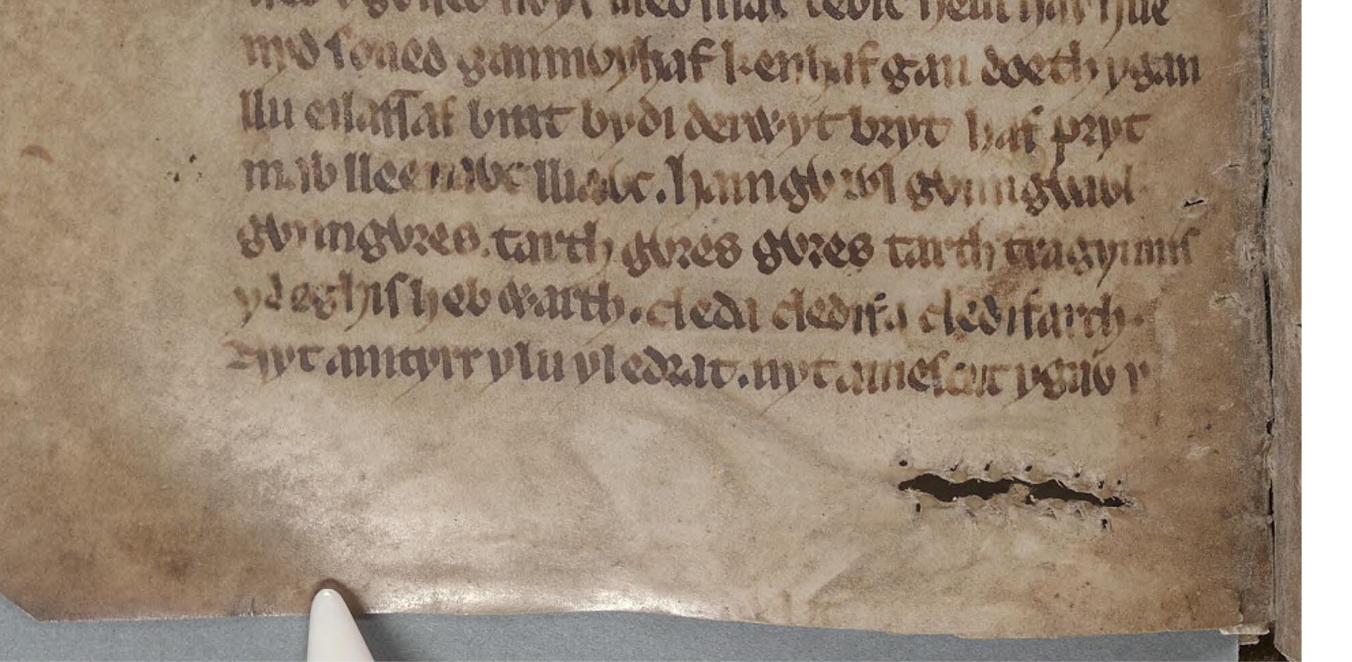
\includegraphics[width=\textwidth]{3orth/images/canvas.png}
%     \caption[The bottom of \acrshort{bt} p.~64]{The bottom of \gls{bt} p.~64. Image credit: The National Library of Wales}
%     \label{fig:p64}
% \end{figure}
The easiest way to account for this situation is that scribe X86  copied the word \mw{kywlat} twice. First, he wrote it as a catchword to make sure the quire starting with page 65 would be placed immediately following the quire ending with page 64. Second, it  is the first word of page 65. In the first instance, he adds orthographic representation of lenition and in the second he copies his exemplar directly. The reason he did not add lenition in the second instance is most likely because he forgot about the syntactic context of this word by the time he had his next quire before him. This instance singularly tells us that scribe X86 was the one who added orthographic lenition to his texts, and that his exemplar did not represent lenition in writing.


\subsection{Sims-Williams}
\label{sec:sims-williams}

\Textcite[107n]{Sim_Buchedd18} writes in his edition of \mw[]{Buchedd Beuno} that `[s]ometimes the radical is written even when lenition is required grammatically, \eg \mw[his patrimony]{y \al{t}reftat ef}; \mw[from exhaustion]{o \al{t}rablinder}; \mw[from this kingdom]{o'r \al{t}eyrnnas honn}'. Here he notices the bare fact that lenition is sometimes not written, and although all his examples start with \mw[]{t},  he does not state that non-lenition may be conditioned by the initial consonant. I found that lenition is not represented twelve times in \mw[]{Buchedd Beuno}, and every single one of these instances starts with \mw[]{t}. This implies that there was a period or an area where lenition of \mw[]{p, c} was written but not \mw[]{t}\footnote{Although I cannot confirm the existence of such a phase in Chapter~\ref{cha:indep-comp-mwbr}, manuscripts \gls{sB}\gls{sE} in Chapter~\ref{cha:welsh-laws} do show noticeably more non-lenition of \mw[]{t} than of \mw[]{p}. In this case, the pattern is muddied by the fact that these manuscripts have complicated textual histories.}.

However, lenition of \mw[]{t} is represented more frequently than it is not. Another saint's life found in the same manuscript  is that of Saint David discussed in Chapter~\ref{cha:stemm-mwbuch-dewi} as \gls{j119}. Here, it is concluded that orthographical lenition of \mw[]{c} was found in the original Welsh composition because it is represented consistently, while lenited \mw[]{p, t} are represented inconsistently, and were therefore added to the text at a later stage. This makes it difficult to pinpoint the time or place when only lenited \mw[]{t} was not represented, because the life of Saint David in \gls{j119} is only a copy of a text which has this pattern, not the text itself. The same must be the case for \mw[]{Buchedd Beuno}.

\subsection{Van Sluis}
\label{sec:van-sluis}
Existential verb \oes\ and the verbal ending \ei\ are noticed by~\textcite{van_development14} as causing lenition to immediately following subjects and objects alike, but not to \mw[]{p, t, c}. This behaviour contrasts with other types of postverbal lenition, such as object lenition and \gls{np} lenition. This pattern is observed in some of the earliest Mabinogion texts, \ie \mow{Culhwch ac Olwen} and \mow{Pwyll Pendefig Dyfed}. These texts are found in the \gls{wbr}, which dates from the mid-fourteenth century, but are thought to have been composed earlier\footnote{\Textcite[43]{rodway_date_2005} dates the composition of \mow[]{Culhwch ac Olwen} to the second half of the twelfth century, but is unsure about \mow[]{Pwyll Pendefic Dyfed}~\autocite[59]{Rod_Where07}. The \gls{wbr} dates to the mid-fourteenth century~\autocite[59]{huws_medieval_2000}.}. The following examples  illustrate the system found in~\textcite{van_development14}:
\begin{mwl}
  \mwc{\acrshort{wbr}~2.2-4}%
  {ac ual ẏ llathrei \al{ỽ}ynnet ẏ cỽn ẏ llathrei \al{c}ochet ẏ clusteu}%
  {And as white as the dogs shone, so red shone their ears.}%
  \mwc{\acrshort{wbr}~481.22}%
  {canẏt oes \al{l}estẏr ẏn ẏ bẏt a dalhẏo ẏ llẏn cadarn hỽnnỽ namẏn hi.}%
  {Since there is no vessel in the world that may keep the strong drink except for this one.}%
  \mwc[storch]{\acrshort{wbr}~483.23}%
  {Nẏt oes \al{t}orch ẏn ẏ bẏt a dalhẏo ẏ gẏnllẏuan namẏn torch canastẏr kanllaỽ}%
  {There is no collar in the world that may hold the leash except for the collar of Canastr Canllaw.}%
\end{mwl}
Because non-lenition of \mw{p, t, c} is found following postverbal contact lenition, but not following object lenition or \gls{np} lenition, \textcite{van_development14} considers this non-lenition a specific feature of \ei\ and \oes\ only; however in light of the difference in orthography between \gls{bbc} and \gls{h}, it may make more sense to think of non-lenition of \mw[]{p, t, c} following \ei\ and \oes\ as an older orthographical stratum, and to think of object and \gls{np} lenition as later innovations to the text\footnote{In fact, \textcite{van_development14} describes how object lenition and \gls{np} lenition gained ground in the \gls{mw} period. Chapter~\ref{cha:welsh-laws} explores how older orthographical strata may be transmitted in later \gls{mw}.}.

\section{Stop orthography as a dating criterion}
\label{sec:lenit-voic-stops-1}
Students of Welsh quickly learn to recognise the difference between \gls{ow} (9th--11th centuries), \gls{mw} (12th--14th centuries) and \gls{mow} (15th century onwards) based on where lenition is represented. \Gls{ow} has no orthographic lenition even though we know it existed in the spoken language, while \gls{mw} does have orthographic lenition, except for \mw{d, rh}. \Gls{mow} has orthographic lenition for all consonants that lenite phonologically, including \mow[]{d, rh}. Thus, a student can easily identify just on the basis of where lenition is represented whether any text before him dates from the \gls{ow} period, the \gls{mw} period, or the \gls{mow} period.

I propose one more intermediate stage between \gls{ow} and \gls{mow}: in early \gls{mw}, lenition of voiceless stops was not represented orthographically word-initially, while in later \gls{mw} it was. Thus, early \gls{mw} texts may be recognised as such because they do not represent lenition of voiceless stops, and late \gls{mw} texts may be recognised as such because they do. This proposal raises the question as to when these lenited voiceless stops came to be represented with \mw[]{b, d, g}. In a text where  lenition is represented orthographically, except for voiceless stops, we may postulate a \lat{terminus ante quem} as well as a \lat{terminus post quem} for its original composition: it must originally have been composed before lenition of voiceless stops was represented orthographically, and after lenition started being represented at all.

One goal of Part~\ref{part:orthography} is to pinpoint more precisely  the origin of orthographical lenition of voiceless stops, so as to more precisely date texts having or lacking this feature. Moreover, \textcite{van_development14} saw that some grammatical environments are particularly conservative in the sense that lack of orthographical lenition may carry over in newer texts. When these environments can be identified, then traces of  earlier orthographical strata in younger manuscripts may be found, which is another goal of Part~\ref{part:orthography}.

\section{Other dating criteria}
\label{sec:other-dating-crit}

It is helpful to compare this task with earlier efforts to date and localise \gls{mw} texts based on linguistic or orthographical criteria. An example of a datable development in Medieval Welsh is the relative frequency of third-person singular preterite indicative ending \mw[]{\mbox{-w(y)s}} and \mw[]{\mbox{-awdd}}. \Textcite{Rod_Datable98} sees a marked increase in the use of \mw[]{\mbox{-awdd}} in the work of thirteenth-century poets compared to their twelfth-century counterparts. Poetry from about 1300 has near-universal \mw[]{\mbox{-awdd}}. He also studied the relative frequency of these markers in prose, and they change in roughly the same period in prose as they did in poetry. \Textcite[68--71]{Rod_Two03} adds to this verbal ending the third-person singular imperfect endings \mw[]{\mbox{-i}} and \ei, the former of which gradually fell out of use during the twelfth and early thirteenth centuries. Still, there was no period in which \mw[]{-i} was more common than \ei. Another such variable is the shift from third-person singular present subjunctive \mw[]{\mbox{-wy/-oe}} towards \mw[]{-o}. \Textcite[71--73]{Rod_Two03} then observes a dramatic rise of \mw[]{\mbox{-o}} in the first half of the thirteenth century, although the situation in poetry is somewhat different from that in prose. The ending \mw[]{-o} was consistently employed as early as the twelfth-century \mow{Braint Teilo}, and \textcite[73]{Rod_Two03} finds only one occurrence of \mw[]{-wy} in prose in \mow[]{Culhwch ac Olwen}. \Textcite{Rod_Where07} provides an example of the way in which the relative incidence of verbal endings may help in creating a rough chronology, and how this methodology compares to other methods in establishing the date and location of medieval literature. The most complete overview of which verbal endings are typical of which period is given by \textcite[166]{rodway_dating_2013}, which shows that compounding insights into the chronology of several developments allows one to date texts with a precision of roughly half a century.

Many of the developments Rodway describes occurred in the thirteenth century and therefore they seem to be roughly contemporaneous with the shift towards representing lenition of voiceless stops. Also, Rodway notices how prose and poetry sometimes, but not always, undergo language change at differing moments, so textual genre may serve as a confounding variable\footnote{I have not found any consistently differing orthographies of lenition between poetry and prose. The difference between the orthography lenition and which verbal ending to use may lie in the fact that the former variable is mostly confined to orthography, while making changes in verbal endings changes poetry when it is spoken as well.}.

%% PSW is not too relevant after all

\Textcite{Tho_Middle93} proposes that linguistic criteria may be used not only for dating the composition of a text, but also for geographic identification. Two of his variables are applicable to this discussion:  stem-formative yod, which may be present or absent, \eg \mw[sureties]{meychyeu/meicheu} as well as stem-formative \mw[]{-th-/-t-} in inflected forms of \mw[with]{gan} and \mw[between]{rwng}, \eg \mw[with him]{ganthaw/gantaw}\footnote{His third variable is third person singular \mw[]{-awd/-ws}, but \textcite{Rod_Datable98}  shows that variation here is chiefly chronological, not dialectal.}. Here, high incidence of yod is associated with north Wales, and low incidence with south Wales. For the inflected prepositions, stem-formative \mw[]{\mbox{-th-}} generally appears in north Wales, and \mw[]{\mbox{-t-}} appears in south Wales. Consequently, there is a strong positive correlation between these features: high frequency of yod implies high frequency of stem-formative \mw[]{\mbox{-th-}}. This research illustrates the value of considering multiple linguistic variables when establishing time and place of composition. If one wishes to establish the place of a text's composition, but the text is too short or lacking in sufficient tokens to judge its dialectal affiliation based on either variable, then one may use both variables to reach a reliable judgment.

The case of stem-formative yod is more complicated than described previously, however. \Textcite{Rus_Celtic90}, for example, notes that variation between \mw[]{\mbox{-awc}} and \mw[]{\mbox{-yawc}} is  lexically conditioned to a great extent, so that incidence of yod in a text does not correlate solely with its geographical origin; incidence of yod is also more frequent in some words or morphemes than other words or morphemes. \Textcite[106]{Wil_Lexical05}  additionally states  that some words show no variation at all, meaning that these items occur with or without yod in both north and south Welsh, and the items that do vary do so according to a pattern reminiscent of lexical diffusion of sound change\footnote{Lexical diffusion occurs when a modification is modified in a subset of a language's lexicon only, and then spreads gradually to other lexical items.}. \Textcite[116]{Wil_Lexical05} then lists fourteen lexical items that occur frequently and show variability regarding presence or absence of yod in his corpus of northern and southern law manuscripts. He notes that the relative frequency of yod has the following order, from low  to high frequency of yod: \mw[relics]{kreir(y)eu} < \mw[pregnant]{beich(y)awc} < \mw[testimony]{tyst(y)olaeth} < \mw[lawful]{kyfreith(y)awl} < \mw[laws]{kyfreith(y)eu} < \mw[witnesses]{tyst(y)on} < \mw[already]{eiss(y)oes} < \mw[try]{keiss(y)aw} < \mw[bullock]{eid(y)on} = \mw[penny]{kein(y)awc} < \mw[sons]{meib(y)on} < \mw[priest]{effeir(y)at} < \mw[eye-witnesses]{gwybyd(y)eit} < \mw[men]{dyn(y)on}. This order means  that \mw[]{kreir(y)eu} appears with yod in relatively fewer instances and in fewer manuscripts than \mw{beich(y)awc} does, for example. \Textcite[117]{Wil_Lexical05} also finds that agreement exists between the texts about the nature of the variation, meaning that one may somewhat confidently predict that a text using yodless \mw[]{meibon} will also use yodless \mw[]{tyston}, because the former item has yod appearing more frequently than the latter. The raw percentages given by \textcite{Tho_Middle93} do not reflect this complexity.

Willis's methodology and observations demonstrate the importance of comparing  manuscript texts that are as similar to each other as possible, except for the variable under study. Chapter~\ref{cha:indep-comp-mwbr} provides a comparison of translations of the same text, and they chiefly differ in the date of their translation into \gls{mw}. Consequently, the different texts under consideration are similar in variables such as genre and vocabulary, but they represent diffent stages of the language. Willis's observations also teach us that the evidential value of a single form containing or not containing yod  differs from word to word. In \mw[]{kreir(y)eu}, for example, yod is quite rare across manuscripts, so a manuscript writing yod is strong evidence for a northern affiliation. Conversely, yodless \mw[]{kreireu} is a more trivial find, so it is not as strong an indicator of southern affiliation. The reverse is the case with \mw[]{effeir(y)at}, where yod is found in a high percentage of instances and a majority of manuscripts have yod; therefore, absence of yod in this word strongly indicates a southern affiliation, while presence of yod is rather trivial. Chapter~\ref{cha:stemm-mwbuch-dewi} discusses how manuscripts may share representation of lenition, or they may share lack of representation. Both types of  instances may be used to argue for a close stemmatic relationship, but the evidential value of represented lenition or its absence depends on the grammatical environment that causes lenition, just as the evidential value of stem-formative yod in establishing dialectal affiliation depends on the word in question.

\section{Overview}
\label{sec:overview}

This section is an overview of the chapters in Part~\ref{part:orthography} and describes the ways they  cumulatively build understanding of the orthographical development of lenited voiceless stops.

Chapter~\ref{cha:some-phon-issu} primarily treats methodological issues. It establishes that a phonological contrast between \lT\ and \xD\ only existed word-initially and thus, only word-initially is there a development to be studied. Therefore, the thesis  only considers word-initial lenition, and not word-medial or word final lenition. This requires a working definition for `word', yet Chapter~\ref{cha:some-phon-issu} finds that a universal definition of `word' is not readily available, and it is perhaps theoretically impossible to define it across languages or across chronolects of a given language. Still, a working definition is reached for the purpose of this thesis. Because primary data in Part~\ref{part:orthography} comprises mostly the presence or absence of orthographical lenition in various \gls{mw} texts,  Chapter~\ref{cha:some-phon-issu} also gives a working definition of lenition. Finally, counting instances where lenition is not written implies exhaustive knowledge of rules governing \gls{mw} lenition. To accomplish this, I discuss the environments  found to cause lenition, and I discuss where non-orthographic lenition is held to exist even though it cannot be seen.

Chapter~\ref{cha:indep-comp-mwbr} establishes a chronology of the developments based on independent thirteenth- and fourteenth-century translations of Geoffrey of Monmouth's \lat{Historia Regum Brittanniae}, where three orthographical stages can be discerned. Up until the mid-thirteenth century, lenited \mw[]{p, t, c} were not represented; in the late thirteenth century, lenited \mw[]{c} was represented, but not \mw[]{p, t}; and in the fourteenth century, all three consonants had lenition represented. The snapshots of orthographical stages provided by these results can be used to date the original composition of hitherto undated texts.

Chapter~\ref{cha:welsh-laws} discusses the orthography of several law manuscripts that contain \mow[]{Llyfr Iorwerth}. Here, the goal is to chart ways that an original composition from before the  thirteenth century is changed as it is copied during the thirteenth century and onwards. The chapter finds that even the most innovative scribes from the fourteenth century preserve traces of older orthography, thus creating a textual form distinguishable from original compositions contemporary with these scribes. Moreover, the chapter explores  alternative ways in which scribes modernised lack of orthographic lenition beyond simply filling in lenition where there was an unlenited consonant previously. Finally, the chapter identifies indicators for comparing lenition in different manuscripts that may be used to argue for a particular stemmatic relationship, providing for the analysis in Chapter~\ref{cha:stemm-mwbuch-dewi}.

Chapter~\ref{cha:stemm-mwbuch-dewi} takes three manuscript witnesses of \mow[]{Buchedd Dewi}, and explores how correspondences or their lack in the orthography of lenition can be used to create a stemma of the various manuscript witnesses and even to allow for the dating of hypothesised nodes in this stemma. 


%%% Local Variables:
%%% mode: latex
%%% TeX-master: "../main"
%%% coding: utf-8
%%% End:
